\chapter{Simulations and Analysis of the 3PWFS}\label{CH4}

To assess the performance of the 3PWFS compared to the 4PWFS, a simulation was developed using the Object Oriented Matlab Adaptive Optics toolbox (OOMAO) \citep{OOMAO}. The OOMAO toolbox is an end-to-end adaptive optics model that can simulate different combinations of guide stars, turbulent atmospheres, wavefront sensors, deformable mirrors, and science cameras. Light is propagated using Fraunhofer diffraction. The master OOMAO toolbox simulates a 4PWFS using Slopes Maps. This chapter details the work that was done to extend OOMAO's utilities to include the 3PWFS and the Raw Intensity signal processing method. We then discuss an experiment performed in OOMAO to study the performance of the 3PWFS compared to the 4PWFS for different magnitude guide stars.

In Section \ref{WFSerror} the SNR for the 3PWFS and 4PWFS was calculated for varying guide star magnitudes. At low light levels when the read noise term dominates the 3PWFS has a gain of $\sqrt{4/3}$ in SNR over the 4PWFS. Other benefits of using a 3PWFS is the simplified manufacturing process. Grinding and polishing a high quality three-sided pyramid optic is faster and cheaper than a four-sided pyramid optic of similar quality. A concern for the 3PWFS is that the wavefront is sampled with three points instead of four. The 3PWFS potential has a larger null space than the 4PWFS, meaning less modes are sensed and the accuracy of the wavefront sensing is reduced. In this and the following chapter we characterize the performance of the 3PWFS in both simulation and on a testbench to explore the potential benefits and disadvantages of the 3PWFS.


\section{The Object Oriented Matlab Adaptive Optics toolbox}

The OOMAO toolbox is a library of classes that are used to assemble objects that simulate different components of an adaptive optics system. The electric field is propagated object to object according to the optical path of the simulated AO system. The main classes include: The source class, atmosphere telescope class, deformable mirror class, pyramid class, and the detector class. The source class generates the beacon guide star used by the AO system for wavefront sensing. The guide star object contains the information of the wavelength bandpass of the system, and the user can set the magnitude of the guide star to change the intensity of light at the detector. The light from the guide star is propagated through the atmosphere to the telescope object. The atmosphere class generates the phase masks that are used to simulate turbulence. The number of layers, the wind speed, Fried parameter $r_0$, and outer and inner scale of the turbulence profile can be set. The resulting phase masks are scaled and compressed into a single phase mask in the pupil plane.  The telescope object defines the aperture of the system, the system resolution, and the exposure time. The default setting is a clear circular aperture, but central obscurations can be modeled from within OOMAO. The user can provide a pupil mask for more complex apertures. The deformable mirror object contains the basis set used for modal wavefront sensing. In the OOMAO library, there are class files to generate Zernike modes and Fourier modes. The number of actuators and the influence function of each actuator can be set by the user. For our simulations, we use a Bezier influence function which is one of the provided influence functions by OOMAO. The pyramid object uses a phase mask to simulate the pyramid tip. The user can select the number of facets, and the apex angle of the pyramid which sets the separation on the WFS detector. The sampling of each of the pupils and the radius of modulation are also user-defined attributes to this object. The detector object records the intensity at the focal plane. At the detector, the user can turn on photon noise, as well as set the read noise for the detector. 

% Listed below is example code to generate the objects in OOMAO.

% \begin{lstlisting}[language=Matlab]
% %% Guide Star
% % Single guide star at infinity, R-band wavelength.
%     ngs=source('wavelength',photometry.R);

% % Science source for Strehl calculation
%     science=source('wavelength',photometry.R);

% %% Atmosphere
% %Fried parameter [m]
%     r0=16e-2;
% %Outer Scale [m]
%     L0=6.25; 
% %Wind speed [m/s]
%     v=7.4;      

% % makes an atmosphere object with the given parameters 
% %at the given wavelength
%     atm=atmosphere(photometry.R,r0,L0,'windSpeed',...
%     v,'windDirection',0);

% %% Telescope
% %Diameter of the telescope in meters
%     D=2  
% %Diameter of the circular entrance pupil in pixels.
% %Sets the sampling of the phase that is generated.
% %Adjust to avoid alaising.
%     nPx=240     
             
% %Frequency in Hz. Sets the integration time and 
% %the simulated loop speed.
%     freq=300    
            

%     tel= telescope(D,'resolution',nPx,...
%     'samplingTime',1/freq);

% %% Deformable Mirror
% %Generates a deformable mirror, that is a grid of actuators 
% %that fill a circular aperture

% %Diameter in actuators of the circular aperture of the DM
%     nAct=9;   
% %Max spatial frequency corrected by the DM
%     d=D/(nAct-1);
%     fmax=1/(2*d); 
% %Max mode # corrected by the DM
%     nMax=ceil(D*fmax/0.37-1);       



% %Zernike basis set
% %Number of modes in the basis set to generate
%     nModes=sum(1:nMax+1)-1;         
% %Zernike basis set generation
% %zern=zernike(2:nModes+1, D, 'resolution', nPx);  
% %Bezier Influence function
%     bif = influenceFunction('monotonic',30/100);    
% %Generates the circular aperture of the DM
%     v=utilities.circle(nAct,nAct);  

% % Deformable mirror object
%     dm = deformableMirror(nAct,...
%         'modes',bif,...
%         'resolution',nPx,...
%         'validActuator',logical(v));

% %% Wavefront Sensor
% %PWFS pupils 20 pixels in diameter
%     nSamp=20 
% %Modulation radius 5 lambda/D
%     mod=5
% %Apex angle of the pyramid. 
% %Sets the separation of pupils
%     alpha=pi/3 
% %Number of sides on the pyramid. 
% %3 and 4 used for simulation.
%     nFaces=3        

% %ngs = guide star object
% %tel= telescope object
% %FWHM in pixels of the focal point spot on the pyramid tip
%     c=2
% %Rotates the pyramid mask to change 
% %orientation of pupils on the detector
%     rotation=3*pi/2

% %Flag that controls what PWFS signal handling method is used. 
% %0 is Slopes Maps, 2 is Raw Intensity. 
% %1 was a failed experiment ignore.
%     altSlopes=0            
% %A flag used to generate an alternative 
% %phase mask for the 3PWFS tip
% %For use on the Spatial Light Modulator on LOOPs. Ignore.                        
%     alternative=0                                       
                        
%     wfs = pyramid(nSamp,nPx,'modulation',mod, 
%     'alpha',alpha,'nFaces',nFaces, 'src',ngs,...
%     'tel',tel, 'c', c,'rotation',rotation,...
%     'altSlopes',altSlopes,... 
%     'alternative', alternative);

% %% Science Camera
% %generates the science camera object with a focal plane 
% %resolution given by the diameter of the telescope aperture.

%     cam=imager('diameter', tel.D);
% \end{lstlisting}



\section{The Pyramid Class}
The master OOMAO toolbox simulates a 4PWFS using Slopes Maps. This section details the changes made to the pyramid class to simulate the 3PWFS. Appendix \label{OOMAOcode} lists the code that is discussed in this section. 


\subsection{The Pyramid Phase mask}
The PWFS is simulated using a single tip/tilt phase mask that is segmented into N parts. The mask is applied in the focal plane to simulate the pyramid tip. In the master OOMAO toolbox, the function that generated the pyramid tip phase mask only generated a 4PWFS mask. To generate the 3PWFS mask, code was adapted from the function that generated the phase masks for the spatial light modulator on the LOOPs testbed. The code was adjusted to have the same scaling as the original mask generator so that a given apex angle gives the same pupil separation for both functions.
\begin{figure}
    \centering
    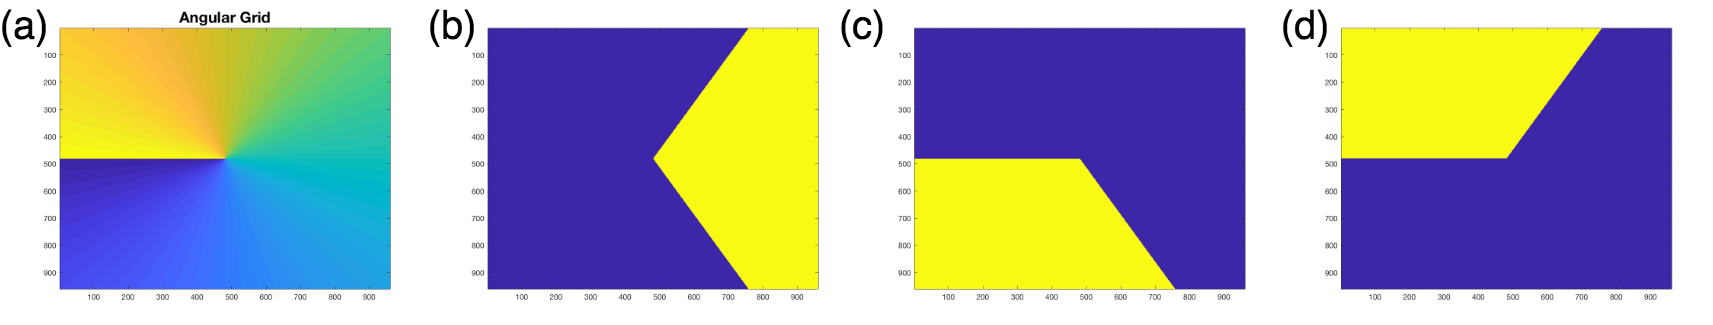
\includegraphics[width=1\textwidth]{Chapter Materials/Chapter Four Materials/phaseMask.png}
    \caption{A. The spiral grid of angular values used to determine where to segments the PWFS facets based on rotation and number of facets. B.C.D. Examples of the binary masks used to segment the pupil plane. Each mask is then given a tip/tilt phase and summed to create the phase mask that simulates the pyramid tip. }
    \label{fig:phaseMask}
\end{figure}

 The mask function works to creates a spiral grid of angular values from $-\pi$ to $\pi$ starting in the center of the frame, as shown in Figure \ref{fig:phaseMask}.A. The grid is used to segment the focal plane corresponding to the number and the rotation of the facets. A mask is made for each facet; and an example of the 3PWFS facet masks are shown in Figure \ref{fig:phaseMask}.B, Figure \ref{fig:phaseMask}.C, and Figure \ref{fig:phaseMask}.D. A tip/tilt phase is added to each of the facet masks and then scaled according to a user inputted apex angle. The masks are then summed to produce the final phase mask for the pyramid tip. Figure \ref{fig:oomaoFigs}.A and \ref{fig:oomaoFigs}.C show the masks for the 3PWFS and 4PWFS. Figure \ref{fig:oomaoFigs}.C and \ref{fig:oomaoFigs}.D shows the resulting pyramid pupils on the simulated wavefront sensor camera, using a flat wavefront and 5 $\lambda/D$ modulation. 

\begin{figure}
    \centering
    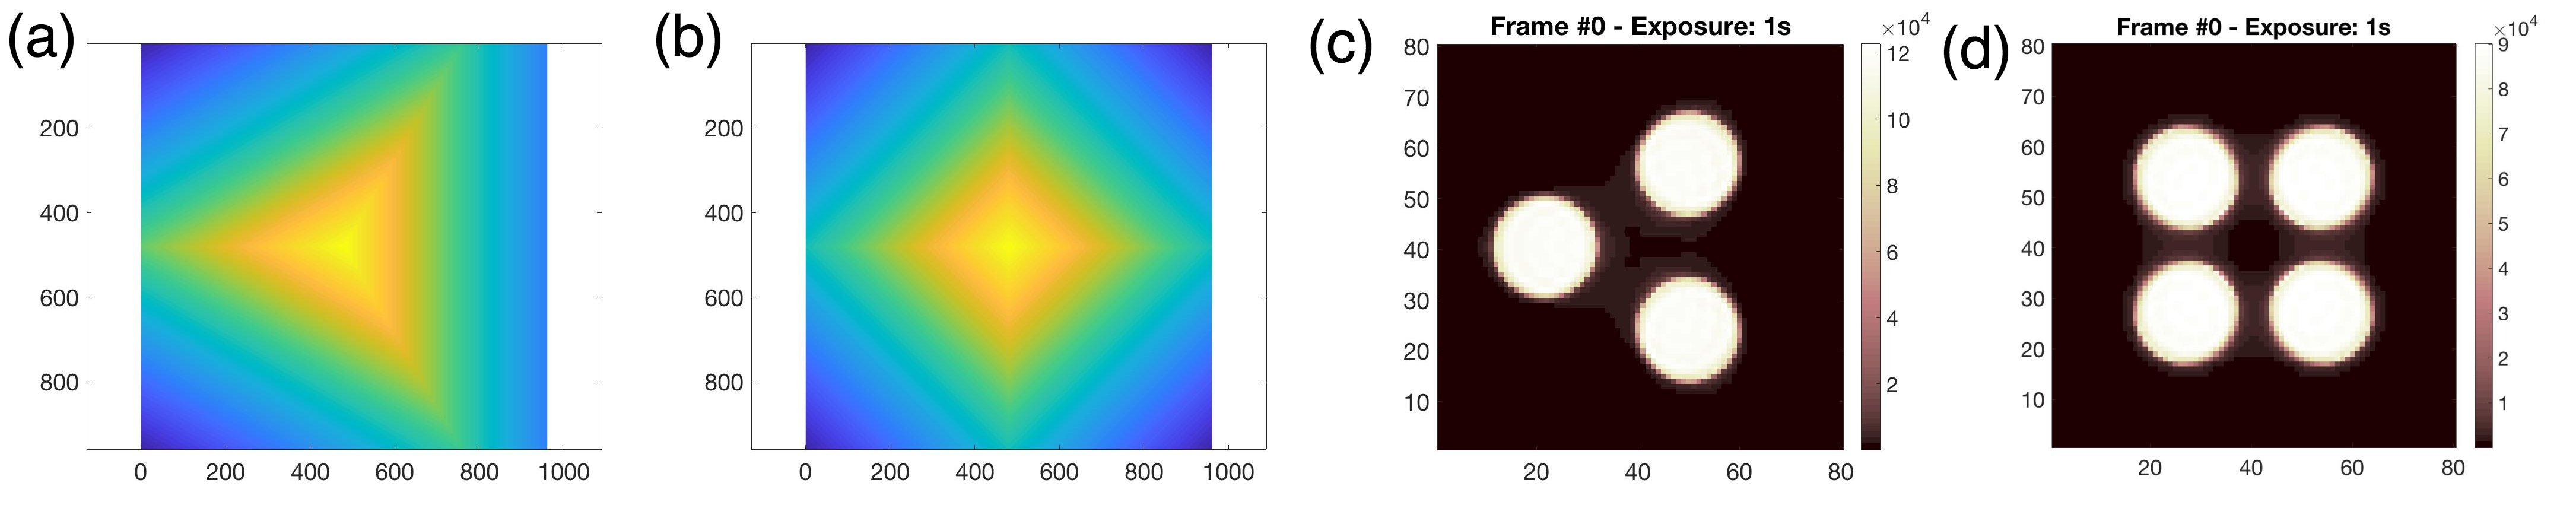
\includegraphics[width=1\textwidth]{Chapter Materials/Chapter Four Materials/oomaoFigs.png}
    \caption{Details of the simulated PWFS in OOMAO. A) and B) The simulated 3PWFS and 4PWFS pyramid masks in OOMAO. These masks are used as a phase mask in the pupil plane to emulate the focal plane splitting and separation done by a real glass pyramid. C) and D) The pupils from the 3PWFS and 4PWFS respectively on the simulated detector. In OOMAO the user can change the size, separation, and intensity values of the pupils through user defined inputs.}
    \label{fig:oomaoFigs}
\end{figure}

\subsection{Signal Handling}

The master OOMAO toolbox simulates a 4PWFS using Slopes Maps. We extended the PWFS class in OOMAO to include the Slopes Maps equations for both the 3PWFS and the 4PWFS, as well as the Raw Intensity method. The pyramid class in OOMAO was hard-coded to expect a matrix size that corresponded to the Slopes Maps signals. For example if the pupils are 20 pixels in diameter, the SM measurement would be a 20x40 matrix, because it produces both a $S_x$ and a $S_y$ measurement. The Raw Intensity signal is a matrix the size of the full frame of the detector. Part of this work was to restructure the pyramid class to accept an arbitrary matrix size.  We included our derivation of the Slopes Maps equation for the 3PWFS derived in Section \ref{Slopes}. For both the Slopes Maps and Raw Intensity method the signal was normalized by the mean value across all valid pixels on the wavefront sensor detector, instead of normalizing pixel by pixel. 

The Slopes Maps calculation requires the knowledge of the location of the pupils on the detector. Each pupil is cropped out and combined with the other pupils for the SM calculation. In the master OOMAO class, the location of the pupil is determined by a calibration step that generates a PWFS with high modulation and a propagated wavefront that contains no phase error. The result is highly uniform pupils on the detector. The detector is split into four quadrants, and each quadrant is thresholded to create a valid detector pixel mask. In the SM calculation, the PWFS signal is divided the same way, and the valid detector pixel mask for each quadrant is applied. This methodology is incompatible with the new way of generating the PWFS masks, which allows for an N-sided pyramid with rotation. A new method of determining the valid detector pixels was developed to be more robust for different PWFS. This method uses the same calibration PWFS. The detector image is thresholded to mask out any pixels with a low signal. The thresholded image is then converted into a binary mask, where the pixels that contain the pupil signals have a value of 1, and all other pixels have a value of 0. Built-in Matlab functions are then used to detect regions, and calculate the centroid of those regions. The resulting binary masks for the 3PWFS and 4PWFS are shown in Figure \ref{fig:pyrcen} A and B. Over-plotted is the location of the calculated centroid given by a dot in the center of each of the regions. OOMAO uses the centroid coordinates to pull out each of the pupils for the SM calculation.

\begin{figure}
    \centering
    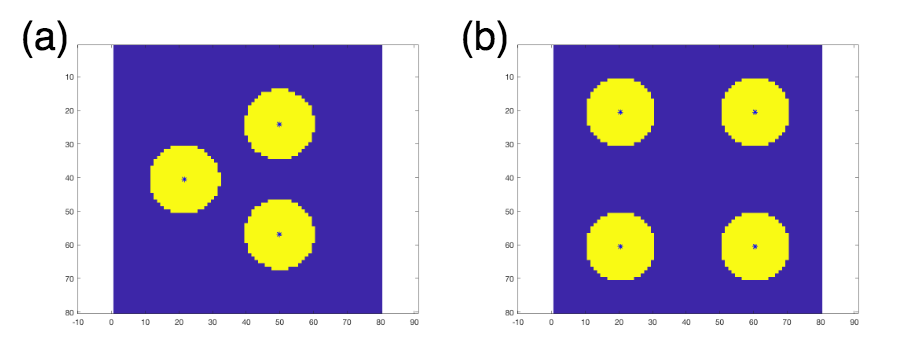
\includegraphics[width=.8\textwidth]{Chapter Materials/Chapter Four Materials/pyramidCenters.png}
    \caption{The calculated binary masks used to detect the location of the pyramid pupils. Over-plotted is the location of the calculated centroid given by a dot in the center of each of the regions.}
    \label{fig:pyrcen}
\end{figure}


\section{Performance Comparison of the 3PWFS and 4PWFS}
\subsection{Simulation}

Using OOMAO an end-to-end simulation of an adaptive optics system was written to compare the performance of the 3PWFS and 4PWFS using both Raw Intensity and Slopes.  The goal was to measure the quality of correction from the AO closed loop by calculating the Strehl Ratio produced by each wavefront sensor as a function of guide star magnitude. In this simulation, the Strehl ratio was calculated using OOMAO's built-in Strehl calculator, which uses the OTF calculated from a PSF with no phase aberration, and a PSF with AO compensated phase aberration. The details of the simulation are summarized in the flow chart in Figure \ref{fig:simulationl}. To characterize the sensitivity of each sensor to read noise the following experiment was performed twice, once at $0.5e^-$ read noise to match that of an OCAM2K camera, and once at $12 e^-$ read noise to match the noisest camera on the Comprehensive Adaptive Optics and Coronagraph Test Instrument (CACTI) at the UA Extreme Wavefront Control Lab (XWCL). Listed below is the experiment performed in OOMAO:

\begin{itemize}
    \item Guide star magnitude was varied incrementally from 0 to 12th magnitude in steps of 2.
    \item At each magnitude closed loop data was taken with different loop gains from 0.1 to 1.8 in steps of 0.1.
    \item At each loop gain the performance was tested by closing the loop on 15 different atmospheric realizations and recording 500 closed loop PSF frames. 
    \item Strehl values were calculated from the PSFs and an average Strehl ratio is reported for a given loop gain at a given magnitude.
    \item The loop gain that gave the highest Strehl value for that guide star magnitude was used in the final calculation of Strehl vs guide star magnitude.
    \item The result is a plot of Strehl versus guide star magnitude, where the value of Strehl has been optimized over the loop gain shown in Figure \ref{fig:overall}
\end{itemize}


\begin{figure}
    \centering
    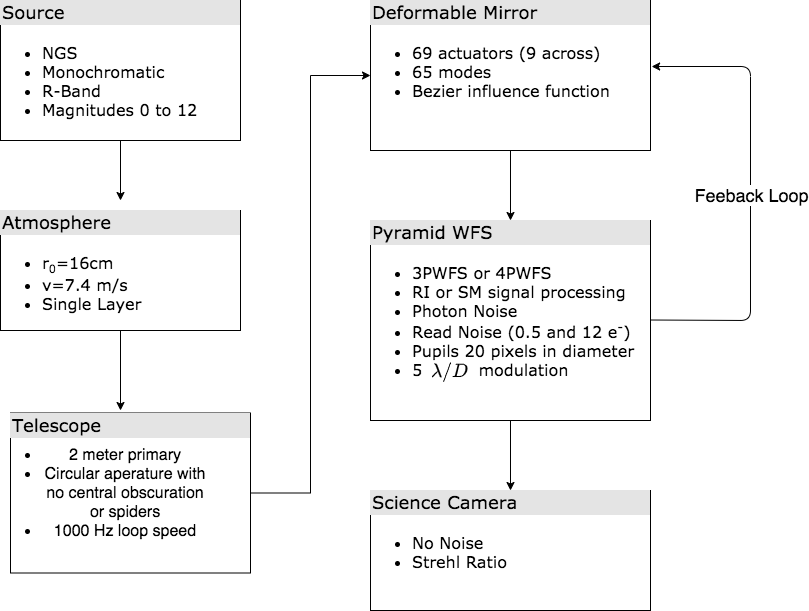
\includegraphics[width=0.8\textwidth]{Chapter Materials/Chapter Four Materials/simulation.png}
    \caption{Experimental details of the simulation done in OOMAO. Light starts at the natural guide star and is propagated through the atmosphere, telescope and wavefront sensor. The wavefront sensor measures a correction that is then applied by the deformable mirror.  The resulting AO corrected PSF is recorded on a noiseless science camera. }
    \label{fig:simulationl}
\end{figure}

\subsection{Results}

In Figure \ref{fig:overall}, no significant difference in performance was found in the comparison case of the wavefront sensors with 0.5$e^-$ read noise. Most on-sky adaptive optics systems use a 4PWFS with Slopes (4PWFS SM) so we use this wavefront sensor as our reference for comparison. The performance of each wavefront sensor was found to be within a percent of Strehl from the 4PWFS SM, across all stellar magnitudes. For the simulations at 12$e^-$ read noise in Figure \ref{fig:overall} a gain of 0.036 Strehl was found for the 3PWFS using Raw Intensity (3PWFS RI) over the 4PWFS SM at a stellar magnitude of 10. At the same magnitude, the 4PWFS RI also outperformed the 4PWFS SM, but the gain was only 0.012 Strehl. This simulation successfully showed the gain in performance from the 3PWFS at low light levels where the effects of read noise are stronger. The overall performance of each wavefront sensor at each guide star magnitude is given in Figure \ref{fig:overall}. In Figures \ref{fig:0RN} and \ref{fig:12RN} comparison plots were made by subtracting the Strehl values for 4PWFS SM from the other wavefront sensors, to help visualize the performance of each wavefront sensor. From these results, we can conclude that the 3PWFS is a viable wavefront sensor with performance comparable to a 4PWFS.


\begin{figure}[h]
    \centering
    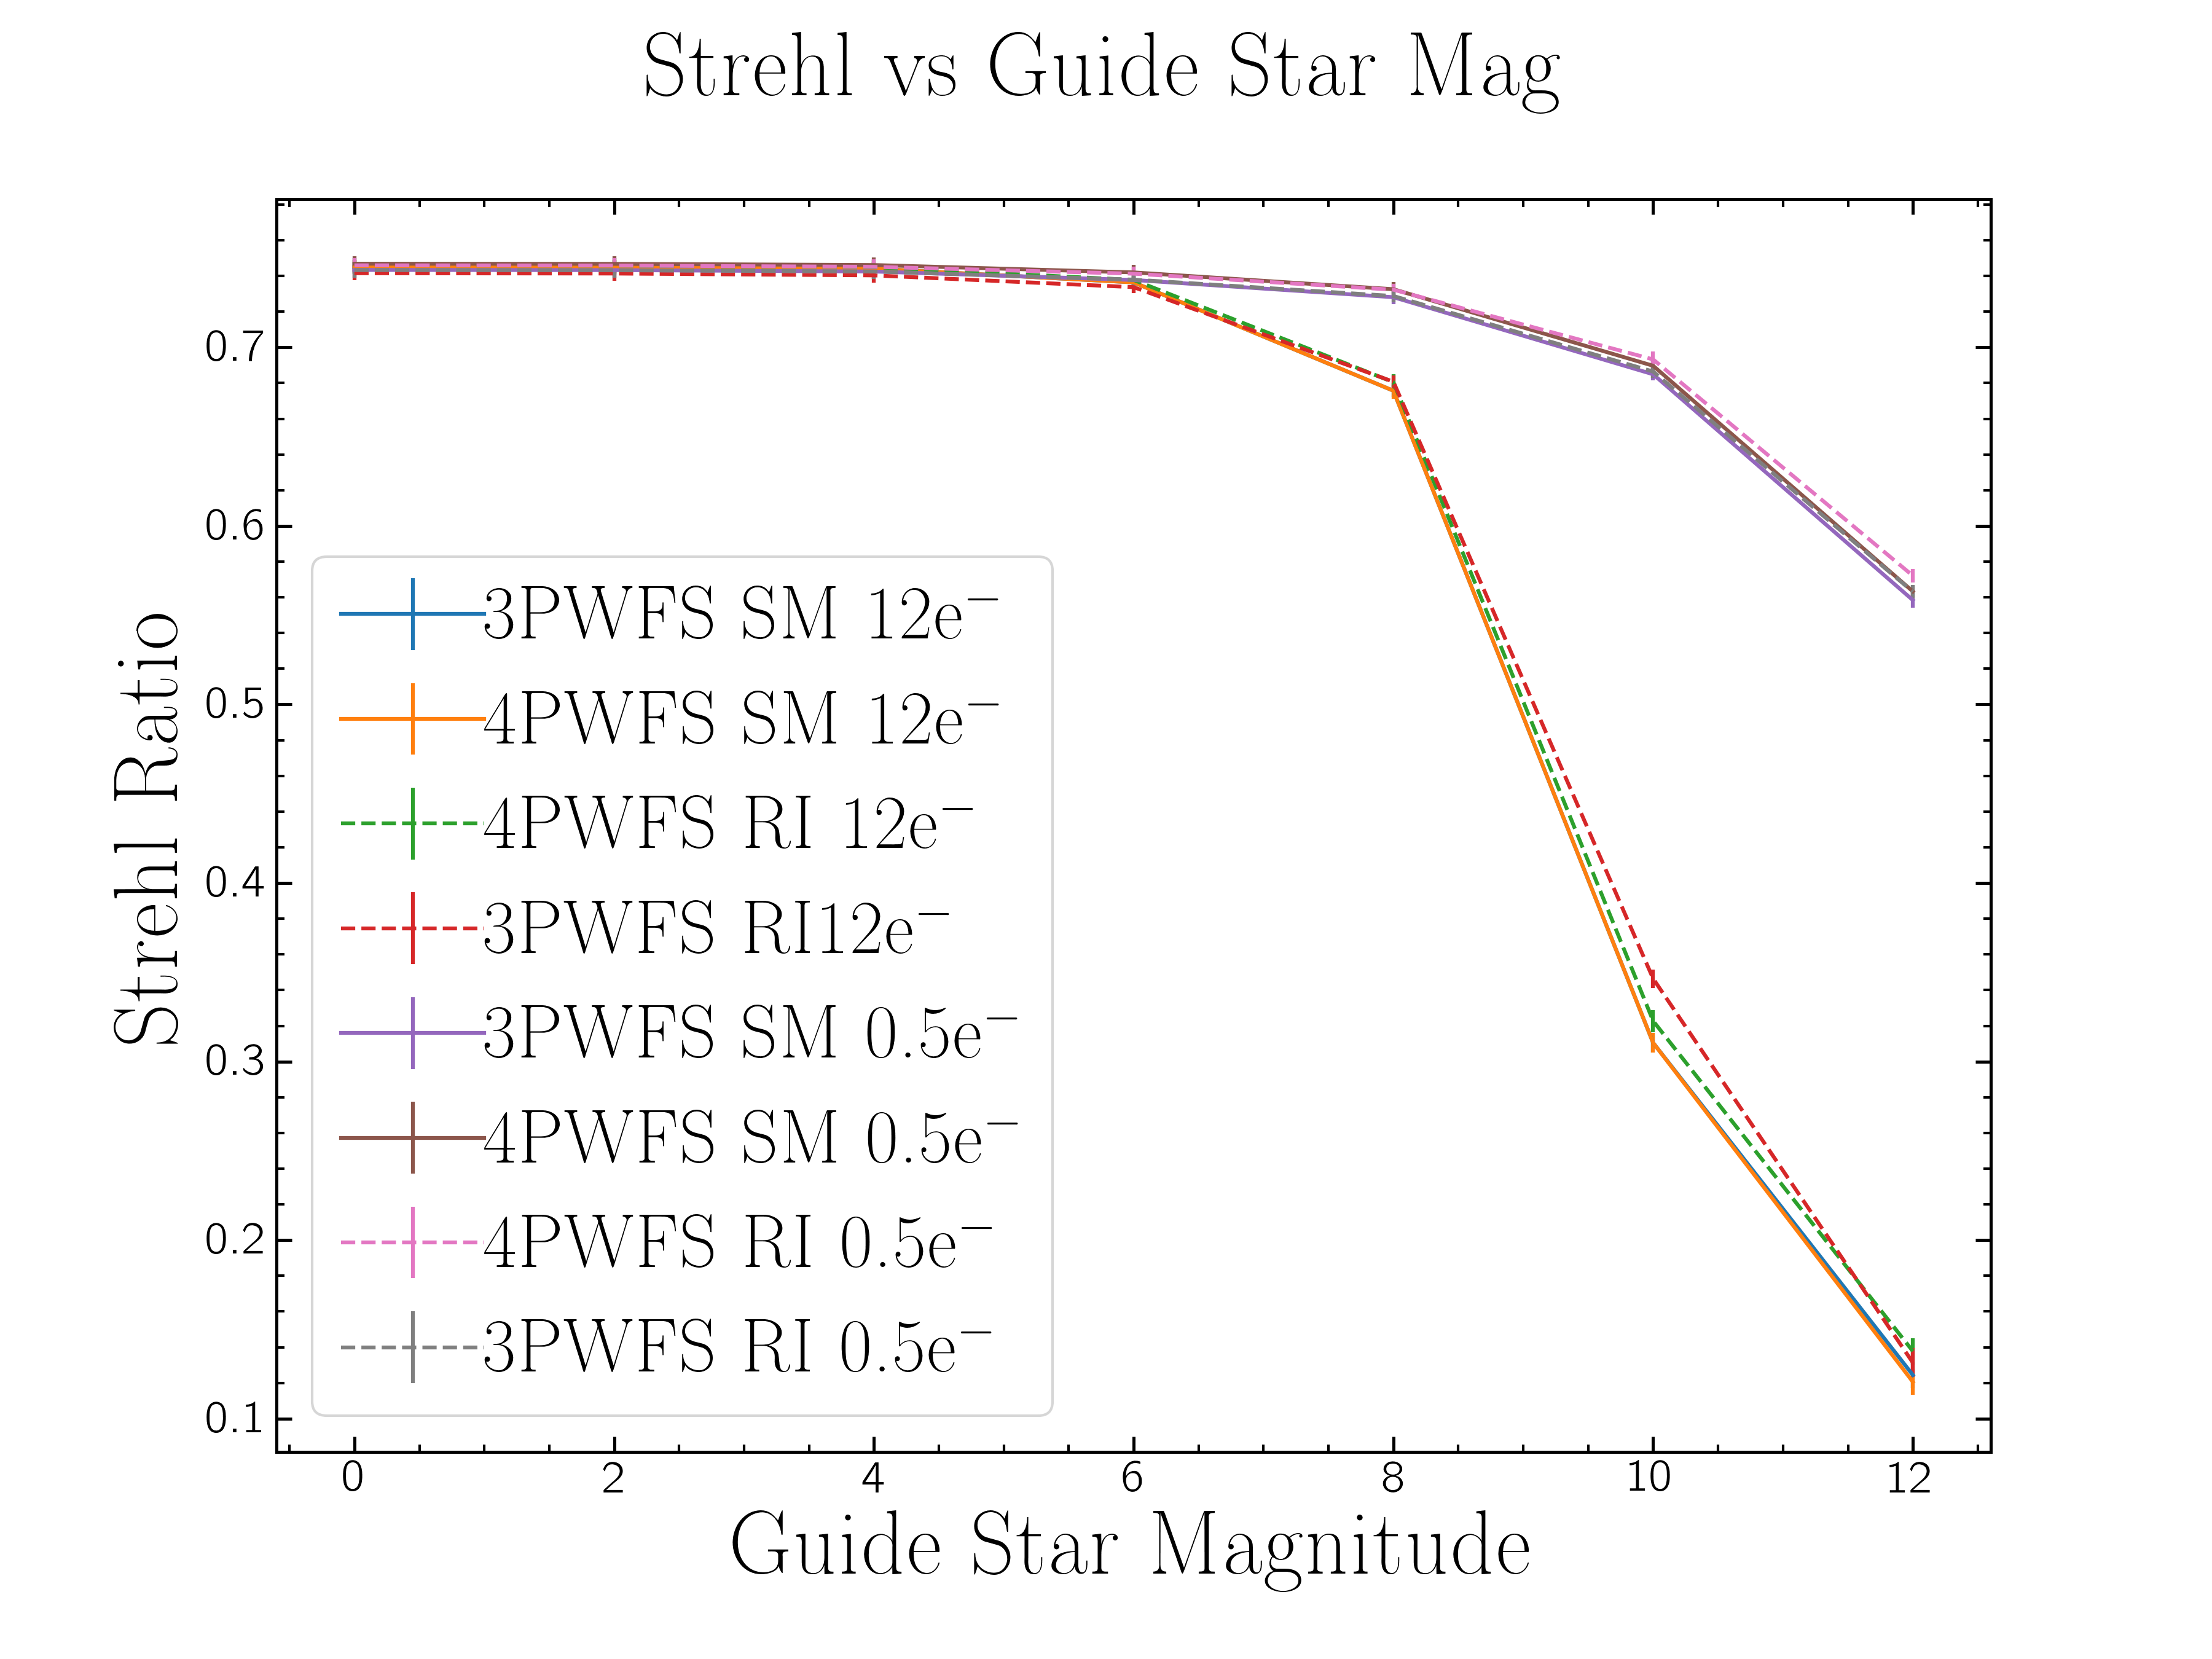
\includegraphics[width=0.8\textwidth]{Chapter Materials/Chapter Four Materials/StrehlvGuideStar4v3.png}
    \caption{Strehl vs Guide Star magnitude for each PWFS. The steep drop off in performance of the lower curves is due to the effects of 12$e^-$ read noise. At guide star magnitude of 10, the read noise starts to matter, and the 3PWFS out performs the 4PWFS. }
    \label{fig:overall}
\end{figure}


\begin{figure}[h]
    \centering
    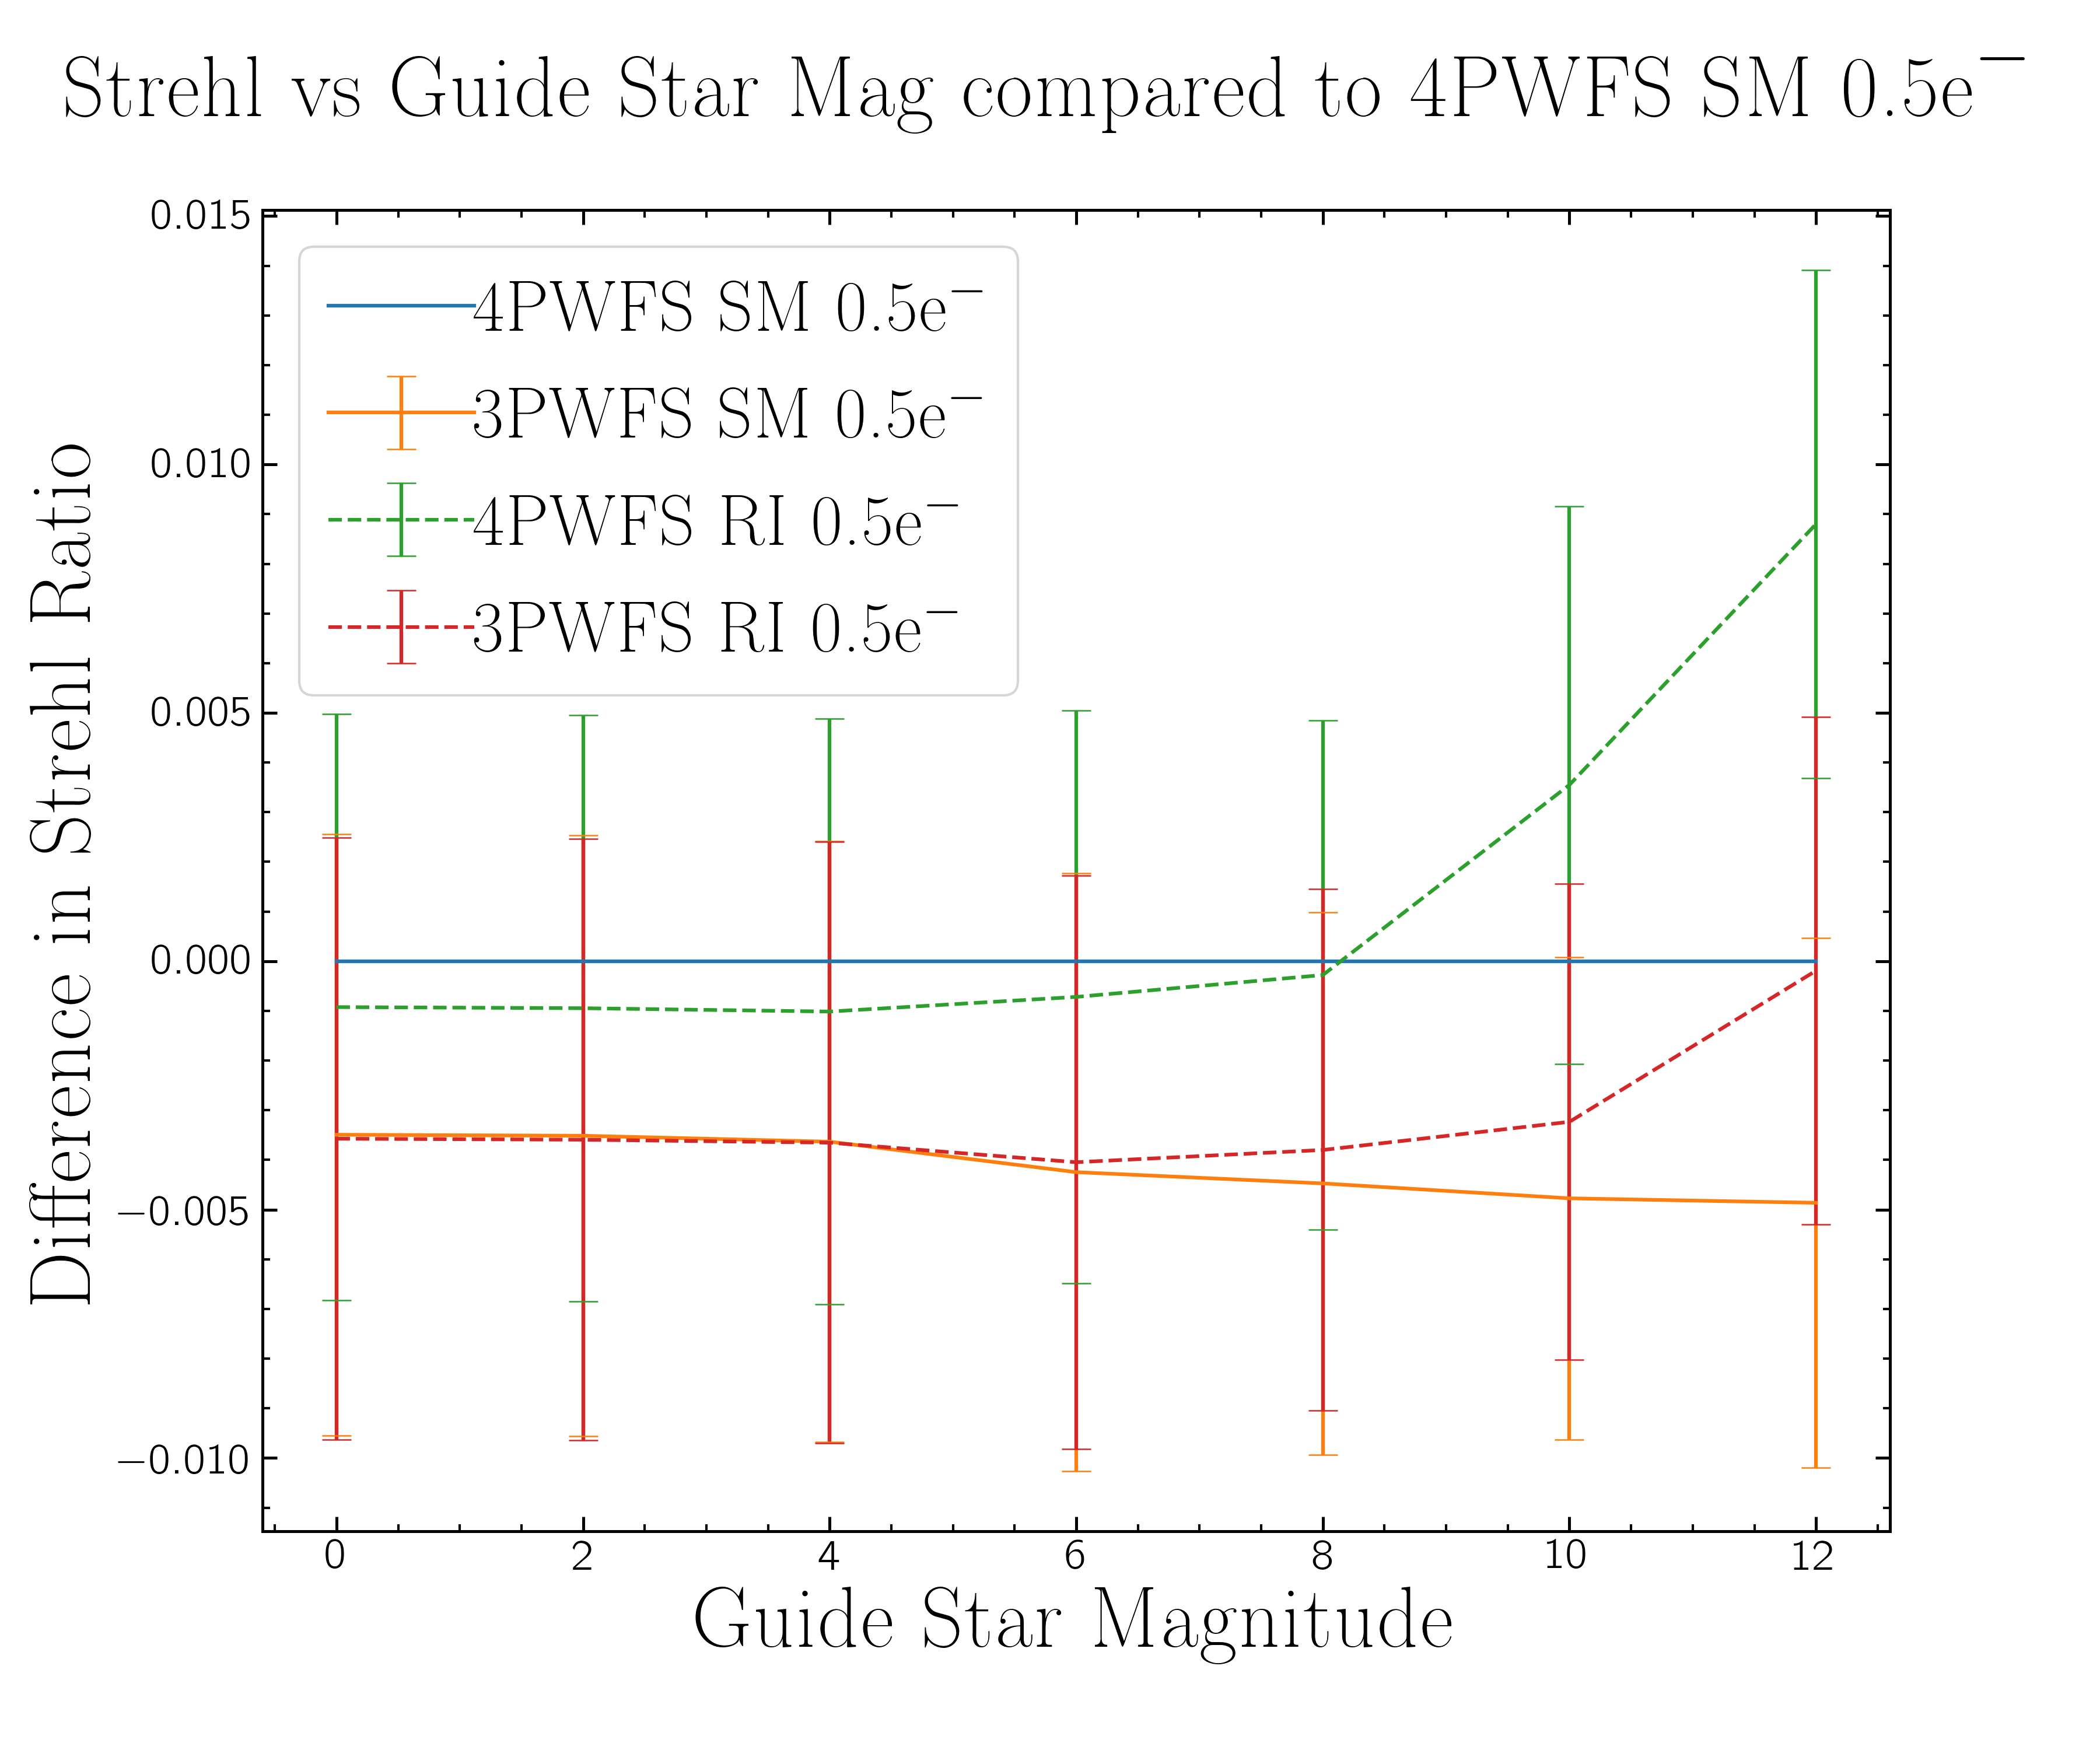
\includegraphics[width=.7\linewidth]{Chapter Materials/Chapter Four Materials/StrehlvGuideStarvs4PWFSRM0e.png}
    \caption{Comparison plot of wavefront sensor performance vs the 4PWFS using Slopes at 0.5 $e^-$ read noise. }
    \label{fig:0RN}
\end{figure}

\begin{figure}[h]
    \centering
    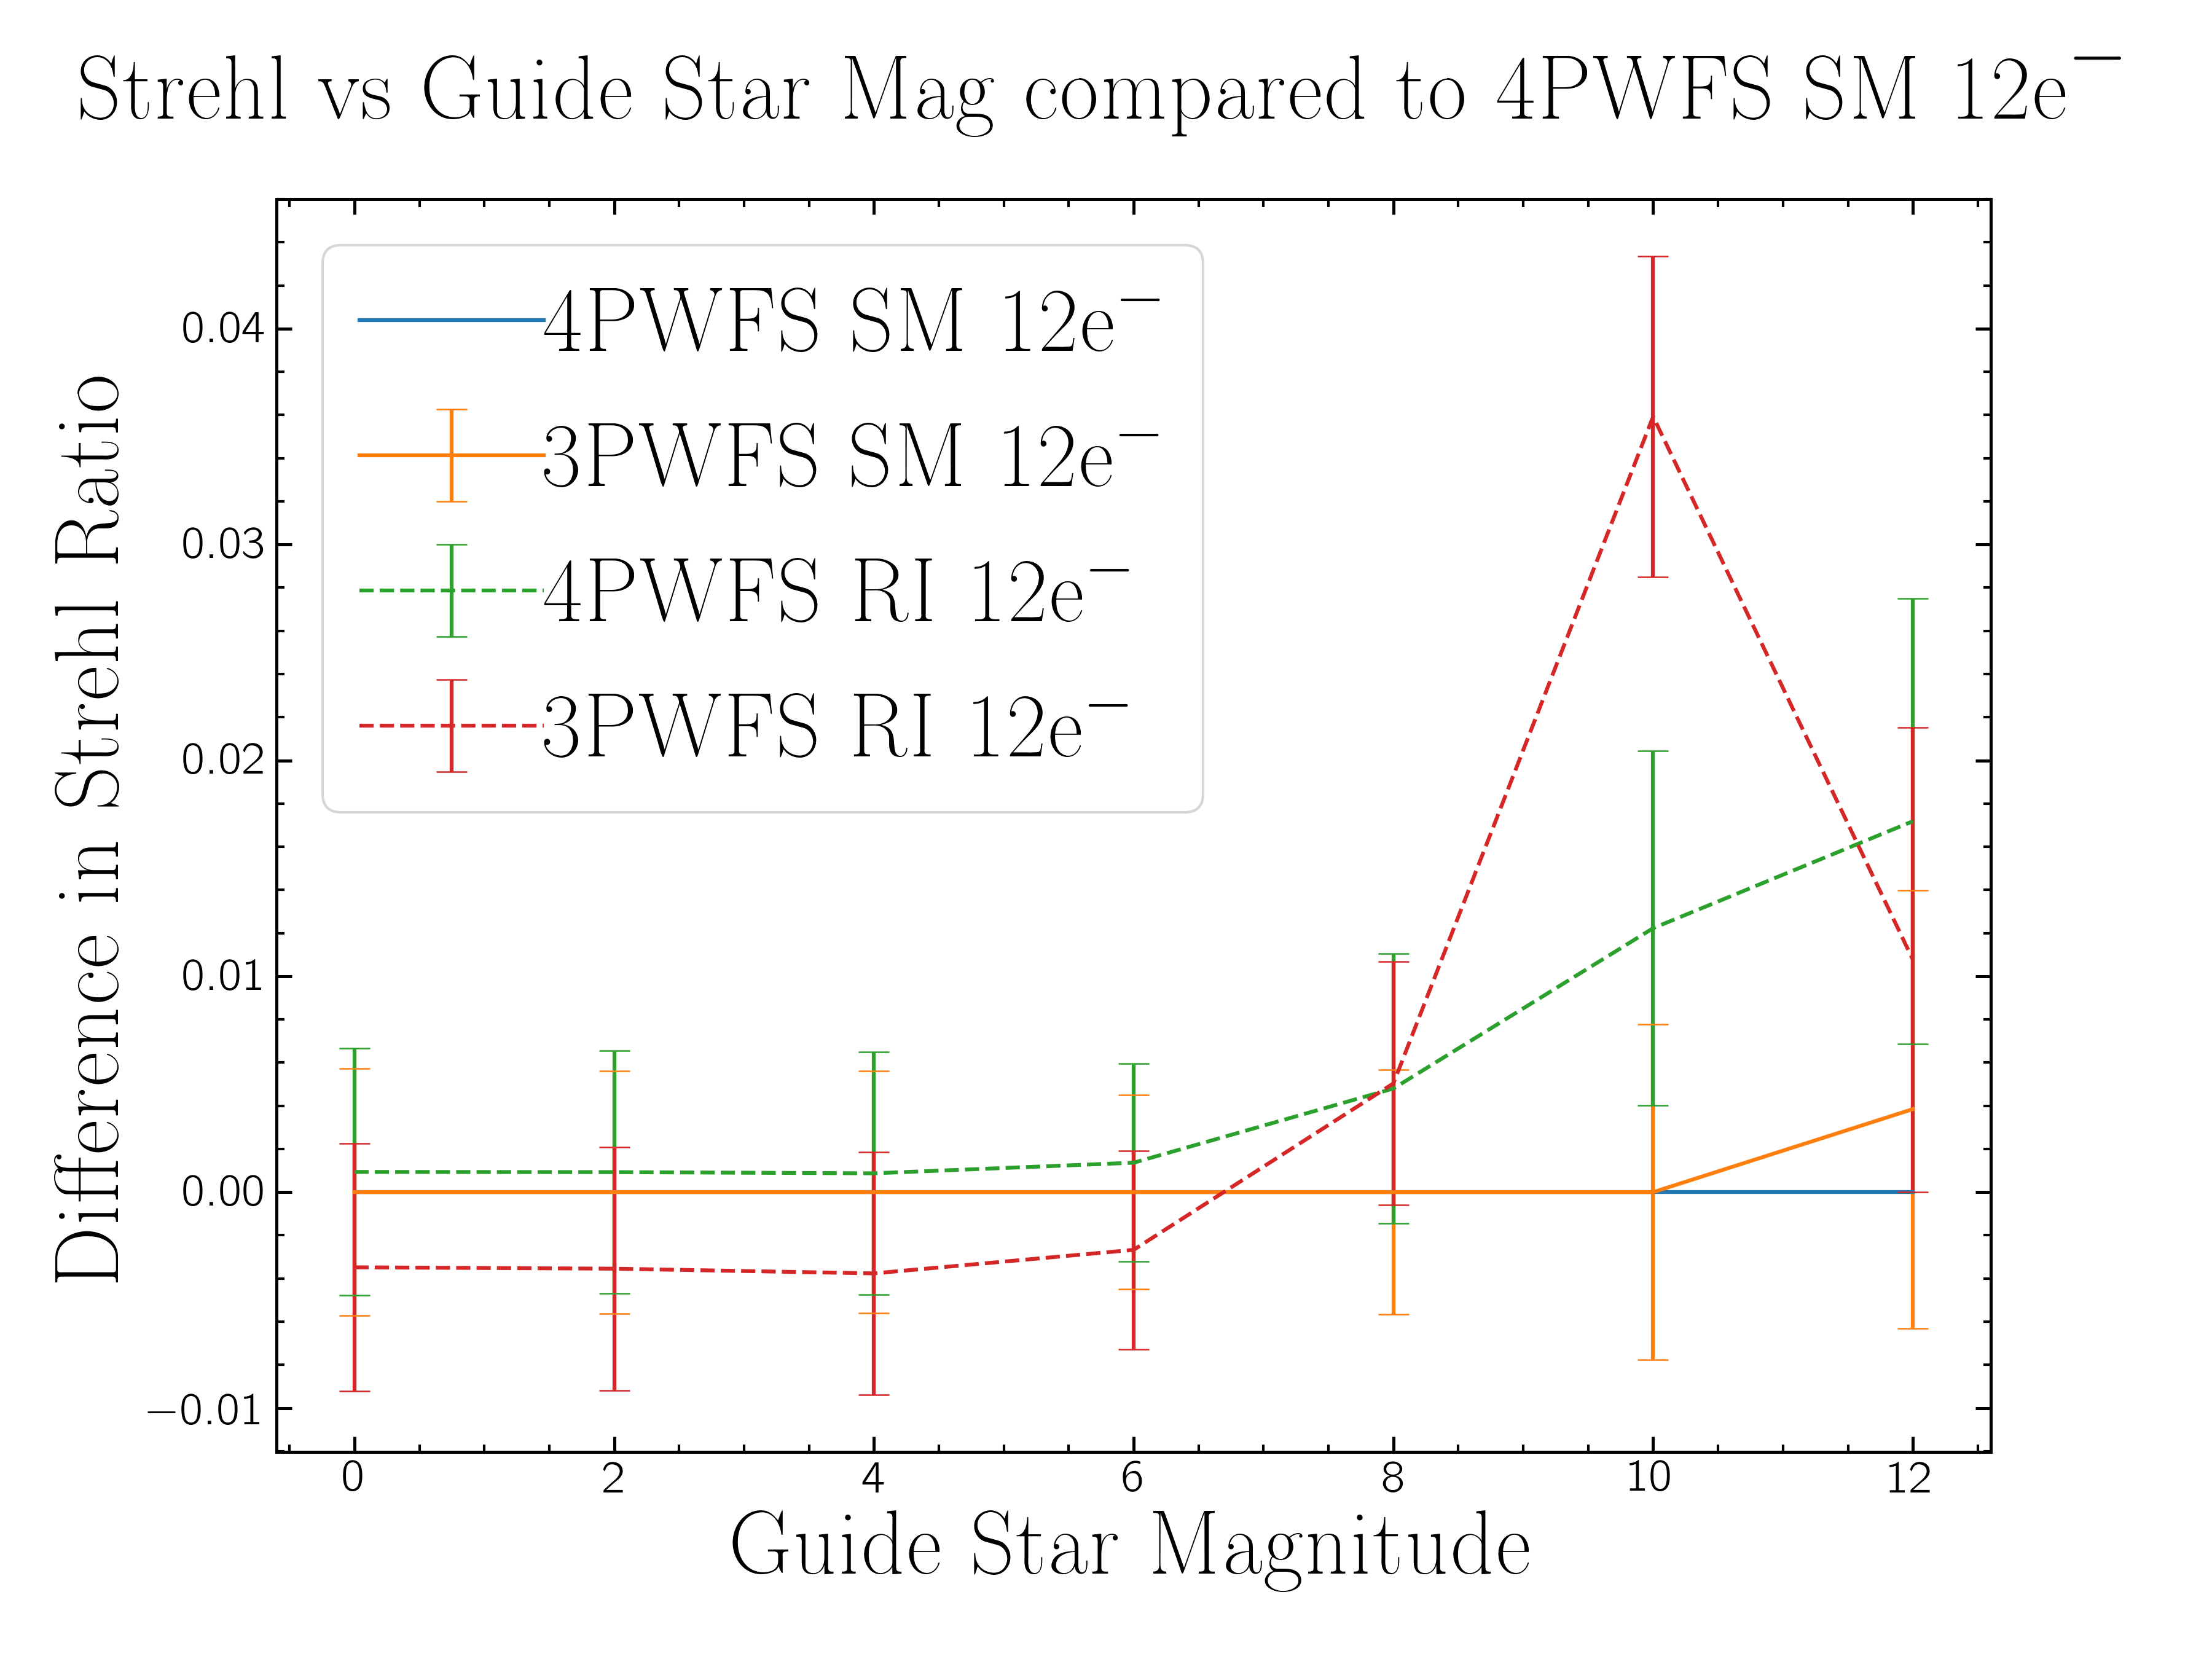
\includegraphics[width=.7\linewidth]{Chapter Materials/Chapter Four Materials/StrehlvGuideStarvs4PWFSRM12e.png}
    \caption{Comparison plot of wavefront sensor performance vs the 4PWFS using Slopes at 12 $e^-$ read noise.}
    \label{fig:12RN}
\end{figure}

\subsection{Discussion}


\cite{codona2018comparative} used the AOsim3 wave optics package to compare end to end performance of a 3PWFS to a 4PWFS with no modulation. In this simulation the Raw Intensity  signal handling method was used. In open loop with no noise the study showed that the 4PWFS out performed the 3PWFS by 0.005 Strehl. Our simulation results agree with the findings by Codona et al. We found in our simulations with 0.5 read noise that the performance of the wavefront sensors are within 0.01 Strehl. Our results differ from Codona et al. when including read noise. They found that for a detector with $3e^-$ read noise, that there was a gap performance improvement by 1 guide star magnitude in favor of the 3PWFS. Codona et. al. considered other factors including system latency, and were sensing in the visible. Our simulations are in r-band and were optimized only for loop gain. Using a detector with $12 e^-$ read noise we found that the performance of the wavefront sensors are once again comparable, and we found only $~0.02$ gain in Strehl from the 3PWFS at 10th magnitude. The scope of our simulations is limited but still agree that the 3PWFS is less sensitive to read noise, however the amount of improvement gained is still under question. Both the 3PWFS and 4PWFS discussed in this paper are refractive, and image all pupils onto the same detector \citep{sanchez2020design}. Moving towards a reflective PWFS that would image each pupil onto its own detector could have a more substantial benefit. Each detector would be smaller, resulting in faster readout speeds with less added read noise. Low read noise detectors are expensive, so using a reflective PWFS would increase system cost and complexity.

\newpage